% 45 minutes including demos of JIT and pkg_composability, exlcluding
% Julia installation.

\documentclass[t]{beamer}
\usepackage{color}
\usepackage{amsmath}
\usepackage{pdfpages}

\definecolor{dkgreen}{rgb}{0,0.5,0}
\definecolor{gray}{rgb}{0.5,0.5,0.5}
\definecolor{Maroon}{rgb}{0.6,0,0}
\newcommand\df{\bf\color{Maroon}}
\newcommand\dff{\bf\color{dkgreen}}
\setbeamercolor{background canvas}{bg=}
%\usetheme{TuringLight}
%\usetheme{TuringDark}

% Presentation data
\title{\color{Maroon} Getting started with Julia and machine learning}
%\subtitle{\small An introduction}
\date{July, 2022}
\author{Anthony Blaom, Samuel Okon}

% Uncomment any of these lines below to set custom size for each of the font sizes.
% The default value is shown in the comment.
%\setlength{\titlefontsize}{6.875\basefontsize}
%\setlength{\subtitlefontsize}{4.375\basefontsize}
%\setlength{\frametitlesize}{2.625\basefontsize}
%\setlength{\framesubtitlesize}{1.625\basefontsize}
%\setlength{\bodytextsize}{2\basefontsize}
%\setlength{\blocktitlesize}{\bodytextsize}
%\setlength{\blockbodysize}{\bodytextsize}

% Start document
\begin{document}

% Title slide (details filled from presentation data fields above)

% \begin{frame}
%   \frametitle{Installing the tutorials}

%   Please follow instructions at:
%   \begin{center}
%     {\df github.com/ablaom/MachineLearningInJulia2020}
%   \end{center}
% \end{frame}

\begin{frame}
        \titlepage
\end{frame}

\begin{frame}
  \frametitle{Interacting}
   Zoom Webinar provides {\bf two} ways to interact:
  
  \begin{block}{Q/A}
    For asking panelists questions
  \end{block}

  \begin{block}{Chat}
    For discussion {\em not} monitored by panelists
  \end{block}\pause

  \begin{block}{\includegraphics[scale=0.1]{raise_hand_forbidden.png}}
  \end{block}

\end{frame}
\begin{frame}
  \frametitle{Outline}
  \begin{enumerate}
  \item Workshop resources
  \item Supervised Learning (mini lecture)
  \item Julia basics 
  \item Data frames 
  \item Supervised Learning using MLJ
  \end{enumerate}
\end{frame}

\begin{frame}
  \vspace{5\baselineskip}
  \begin{center}
  {\Large machine learning $\ne$ deep learning\\
  \mbox{}\hspace{4cm} \pause {\normalfont (neural networks)}}
  \end{center}
\end{frame}

\begin{frame}
  \frametitle{A plethora of machine learning models}
  \begin{center}
    \includegraphics[scale=0.25]{plethora_of_models.png}
  \end{center}
  {\tiny Figure source: Oleksii Trekhleb ({\ttfamily https://github.com/trekhleb/homemade-machine-learning})}
\end{frame}

% \iffalse

\begin{frame}
  \frametitle{Introducing Julia}
  Julia is an open source, general-purpose programming language, in
  the fourth year of its first {\df stable} release 1.0.\pause

  \begin{block}{Key take aways}
    \begin{itemize}
    \item Julia let's you write {\df fast}
      code {\df fast}.\pause
    \item Maximally hackable.
  \end{itemize}
  \end{block}
\end{frame}

% lego analogy
\includepdf[scale=1.3,pages={1,3}]{lego.pdf}


\begin{frame}
  \frametitle{Introducing Julia}
  Julia is an open source, general-purpose programming language, in
  the fourth year of its first {\df stable} release 1.0.

  \begin{block}{Key take aways}
    \begin{itemize}
    \item Julia let's you write {\df fast}
      code {\df fast}.
    \item Maximally hackable.
    \item Julia's design makes {\df extending} Julia code easy,
      promoting a relatively rapid expansion of third party libraries.
    \end{itemize}
  \end{block}
\end{frame}

\begin{frame}
  \frametitle{Julia's secret sauce}
    \begin{itemize}
    \item {\df Just-in-time compilation}
    \item {\df Multiple dispatch}
    \item {\df Abstract type system} (typing is dynamic, nominative and parametric)
  \end{itemize}
\end{frame}

\begin{frame}
  \begin{block}{Workshop resources:}
    {\large\texttt{github.com/ablaom/HelloJulia.jl}}
    \end{block}
\end{frame}

\begin{frame}
  \begin{block}{Secret sauce demo:}
    {\large\texttt{github.com/ablaom/HelloJulia.jl/}}\newline
    {\large\texttt{blob/dev/demos/secret\_sauce/notebook.ipynb}}
    \end{block}
\end{frame}
%
\begin{frame}
  \begin{block}{Package composability demo:}
    {\large\texttt{github.com/ablaom/HelloJulia.jl/}}\newline
    {\large\texttt{blob/dev/demos/pkg\_composability/notebook.ipynb}}
    \end{block}
\end{frame}

\begin{frame}[plain]
  %  \begin{center}
     \includegraphics[scale=0.25]{mandel.png}
%   \end{center}
\end{frame}
% stars
\begin{frame}[plain]
  %  \begin{center}
     \includegraphics[scale=0.30]{julia_stars.png}
%   \end{center}
\end{frame}

% 2018 conference (2021: 3 x talks, 50 x registration):
\includepdf[pages=10]{Sebastian.pdf}

% growth stats 2020 - 2021:
\begin{frame}[plain]
  %  \begin{center}
     \includegraphics[scale=0.70]{julia_stats.png}
%   \end{center}
\end{frame}

% high profile applications:
\includepdf[pages=18-21]{julia_for_ecologists.pdf}
\includepdf[pages=23]{julia_for_ecologists.pdf}

% \begin{frame}
%   \frametitle{The Two Language Problem}
%   \begin{itemize}

% \item   Older programming languages like C and FORTRAN are designed to {\em
%     run} fast. Almost all {\df computationally demanding} tasks
%   (weather forecasting, machine learning, etc) are performed by
%   calling code written in these languages. \pause

% \item ``Scripting'' languages like python, MATLAB, and R allow you
%   quickly {\df wrap} computational tasks into {\df customized and easily
%     modified workflows}. They also accelerate {\df testing and
%     protyping} of new computational algorithms.\pause

% \item These languages are {\df too slow} for computationally intensive tasks.
% \end{itemize}
% \end{frame}

\begin{frame}
  \frametitle{Popular libraries (packages)}
  These are all pretty mature:
  \begin{itemize}
  \item DataFrames.jl and CSV.jl  - {\df in-memory data manipulation}
  \item Plots.jl (also easy to call R's ggplot())
  \item $\star$ JuMP.jl - {\df constrained optimization}
  \item $\star$ DifferentialEquations.jl
  \item StatsModels.jl, GLM.jl - {\df traditional stats models}
  \item Flux.jl  - {\df deep learning}
  \item $\star$ Turing.jl, Soss.jl, ... {\df probabilistic programmming}
  \item MLJ.jl - multi-pardigm {\df machine learning} platform
  \item Pluto.jl - {\df ``reactive'' notebooks}
  \end{itemize}
\end{frame}

% lines of code versus mean run time:
\includepdf[pages=11]{julia_for_ecologists.pdf}

\begin{frame}
  \frametitle{Why  is two languages a problem ?}
  \begin{itemize}
    \item Can't easily {\df modify} core algorithms
    \item Barrier to {\df understanding algorithms} even if not seeking to modify them
    \item Complicates installation of a complete software stack
    (package {\df dependency hell}, manual interventions)
    \item Barrier to {\df transparency} and {\df reproducibility}
    \item {\df Hampers innovation}, development of novel algorithms
    \item Barrier to {\df composing libraries} (e.g., automatic differentiation)
  \end{itemize}
\end{frame}

% slows innovation engineers <--> researchers
\includepdf[scale=1.3,pages={1,2,4}]{slows_innovation.pdf}

\begin{frame}[plain]
  \frametitle{Fast code written fast: DifferentialEquations.jl}
  % \frametitle{DifferentialEquations.jl}
  %  \begin{center}
     \includegraphics[scale=0.27]{de_solver_software_comparsion.pdf}
%   \end{center}
\end{frame}

% % data science pipeline
% \includepdf[pages=3-5]{Sebastian.pdf}

% \begin{frame}[plain]
%     \includegraphics[scale=0.45]{benchmarks.png}
% \end{frame}


% \begin{frame}
%   \frametitle{The Expression Problem}
%   As in any kind of architecture, the central concerns of a
%   programming language are {\df form} and {\df function}. Roughly
%   speaking, the {\df Expression Problem} is the problem of how to
%   represent data (form) and how to articulate required behaviour
%   (function) in way that allows {\df extension} of both in an optimal
%   and safe way.\pause
%   \begin{itemize}
%     \item Object oriented languages typically score poorly here (Ruby has a
%       dirty way, Scala a clean workaround).
%     \item Julia scores well. {\df Proof:} \pause Large code-reuse, package composibility
%   \end{itemize}
% \end{frame}


\begin{frame}
  \frametitle{Other features}
  \begin{itemize}
    \item Fast user-defined composite types (C-like structs)
    \item Lisp-like macros/metaprogramming
    \item Call C functions directly
    \item Can wrap Python, R Java/Scala
    \item State-of-the-art distributed computing and multi-threading support
  \end{itemize}
\end{frame}

% code snippet:
\begin{frame}
  \frametitle{Other features (continued)}
  \begin{itemize}
  \item First-class math support
    \item Exellent REPL (console)
    \item Built-in package manager
    \item Automatic differentiation (Zygote.jl)
  \end{itemize}
\end{frame}

\begin{frame}
  \frametitle{Drawbacks}
  For most users all serious drawbacks derive from Julia's young age:
  \begin{itemize}
     \item Smaller number of libraries
     \item Smaller community of users
     \item Some interfaces and tooling less polished
     \item More bugs (in libraries, few in language itself)
  \end{itemize}
  Other drawbacks and annoyances:
  \begin{itemize}
     \item Limited support for exporting programs as stand-alone executables.
     \item The ``time to first plot'' problem.
  \end{itemize}
\end{frame}


% %% Intro to machine learning process

%\fi

\begin{frame}
  \frametitle{Supervised Learning}
  Learning to {\df predict} some target variable {\df\large y} from a
  knowledge of some other variables {\df \large X} (the {\it input features}).\pause
  \begin{table}
  \begin{tabular}{|l|l|}
    \hline
    ${\mathbf X}$  & ${\mathbf y}$ \\ \hline
    longitude, latitude, temperature, pressure & wind speed \\
    individual DNA gene sequence & got diabetes\\
    word frequencies in email & is junk? \\
    an image of handwritten digit & $0, 1, 2, \ldots, 8$ or $9$ \\
    num rooms, floor area, zip code & selling price \\
    {\bf Titanic:} sex, class, fare, where embarked & survived? \\
    \hline
  \end{tabular}
  \end{table}
\end{frame}

\begin{frame}
  \frametitle{Supervised Learning}
  Learning to {\df predict} some target variable {\df\large y} from a
  knowledge of some other variables {\df \large X} (the {\it input features}).
  \begin{center}
    \includegraphics[scale=0.17]{X.png}\mbox{~~~~}
    \includegraphics[scale=0.17]{y.png}
  \end{center}
\end{frame}

\begin{frame}
  \frametitle{Supervised Learning}
   \begin{center}
    \includegraphics[scale=0.6]{overfitting1.png}
   \end{center}
\end{frame}

\begin{frame}
  \frametitle{Supervised Learning}
   \begin{center}
    \includegraphics[scale=0.6]{overfitting2.png}
   \end{center}
\end{frame}

\begin{frame}
  \frametitle{Supervised Learning}
   \begin{center}
    \includegraphics[scale=0.6]{overfitting3.png}
   \end{center}
\end{frame}

\begin{frame}
  \frametitle{Supervised Learning}
   \begin{center}
    \includegraphics[scale=0.6]{overfitting4.png}
   \end{center}
\end{frame}

\begin{frame}
  \frametitle{Supervised Learning}
   \begin{center}
    \includegraphics[scale=0.6]{overfitting5.png}
   \end{center}
\end{frame}

\begin{frame}
  \frametitle{Supervised Learning}
   \begin{center}
    \includegraphics[scale=0.6]{overfitting6.png}
   \end{center}
 \end{frame}

 \begin{frame}
   \frametitle{Supervised Learning}
   \begin{block}{Setup}
     Got historical data with:
     \begin{itemize}
     \item {\df features}  $X$ (aka, inputs, patterns)
     \item {\df target} $y$ (aka, labels)\pause
     \end{itemize}
   \end{block}
   \begin{block}{Basic machine learning workflow}
     \begin{enumerate}
     \item Split historical data into {\df training} and {\df test} sets.\pause
     \item Train the model using the {\df training} set\pause
     \item Get model predictions $\hat y$ given $X$ for {\df test} set.\pause
     \item Compare $\hat y$ with $y$ from the {\df test} set using some {\df measure} (e.g.,
       mean squared error).\pause
     \item Change hyperparameters of model and repeat.
     \end{enumerate}
   \end{block}
 \end{frame}

\begin{frame}[plain]
  \begin{center}
     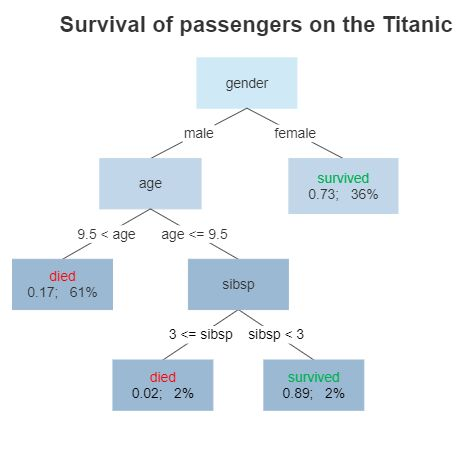
\includegraphics[scale=0.55]{titanic_tree.jpg}
   \end{center}
\end{frame}



\end{document}

%%% Local Variables:
%%% mode: latex
%%% TeX-master: t
%%% End:
